\documentclass[tikz,border=2pt]{standalone}
\usepackage[T1]{fontenc}
\usepackage{libertine}
\usepackage{xcolor}
\usetikzlibrary{arrows.meta,calc,positioning}

\begin{document}
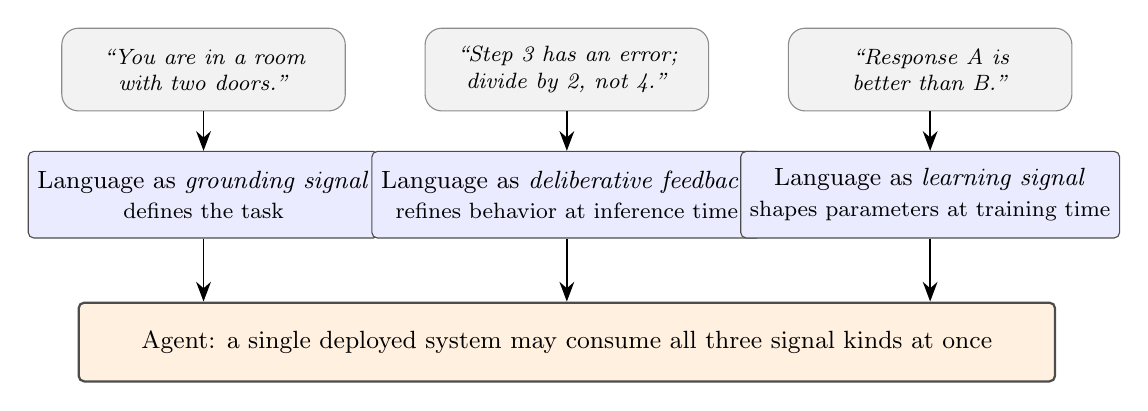
\begin{tikzpicture}[
    font=\small,
    example/.style={draw=black!45, rounded corners=6pt, align=center, minimum width=3.6cm, minimum height=1.05cm, fill=black!5, font=\footnotesize\itshape},
    role/.style={draw=black!70, rounded corners=2pt, align=center, minimum width=3.6cm, minimum height=1.1cm, fill=blue!8},
    agent/.style={draw=black!70, thick, rounded corners=2pt, align=center, minimum width=12.4cm, minimum height=1.0cm, fill=orange!12},
    sig/.style={-{Stealth[length=2.5mm]}, semithick}
]
    \node[example] (ex1) {``You are in a room\\with two doors.''};
    \node[example, right=1.0cm of ex1] (ex2) {``Step 3 has an error;\\divide by 2, not 4.''};
    \node[example, right=1.0cm of ex2] (ex3) {``Response A is\\better than B.''};
    \node[role, below=0.5cm of ex1] (r1) {Language as \emph{grounding signal}\\\footnotesize defines the task};
    \node[role, below=0.5cm of ex2] (r2) {Language as \emph{deliberative feedback}\\\footnotesize refines behavior at inference time};
    \node[role, below=0.5cm of ex3] (r3) {Language as \emph{learning signal}\\\footnotesize shapes parameters at training time};
    \draw[sig] (ex1) -- (r1);
    \draw[sig] (ex2) -- (r2);
    \draw[sig] (ex3) -- (r3);
    \node[agent, below=0.8cm of r2] (agent) {Agent: a single deployed system may consume all three signal kinds at once};
    \draw[sig] (r1.south) -- (r1.south |- agent.north);
    \draw[sig] (r2.south) -- (agent.north);
    \draw[sig] (r3.south) -- (r3.south |- agent.north);
\end{tikzpicture}
\end{document}
